%% Nature "Matters Arising" — Springer Nature template (sn-jnl, sn-nature style)
%% Arising from: M. Pachitariu et al., Nature (2026).
%%
%% V5 — COMPRESSED submission version (target main text <=1200 words).
%%   Single throughline: the two reported observables do not identify the
%%   proposed symmetric-critical mechanism. Math/derivations and the full
%%   FlyWire test live in the Supplementary Information. Two display items.
\documentclass[pdflatex,sn-nature]{sn-jnl}

\usepackage{graphicx}
\usepackage{amsmath,amssymb,amsfonts}

\newcommand{\alphaeff}{\alpha_{\mathrm{eff}}}
\newcommand{\asym}{\mathcal{A}}

\raggedbottom

\begin{document}

\title[Identifiability of symmetric criticality from population activity]{%
Cortical population activity does not identify symmetric critical dynamics}

\author[1,2]{\fnm{Mingyi} \sur{Huang}}\email{myhuang20@fudan.edu.cn}

\author*[1,2]{\fnm{Yuguo} \sur{Yu}}\email{yuyuguo@fudan.edu.cn}

\affil*[1]{\orgdiv{Research Institute of Intelligent and Complex Systems, State
Key Laboratory of Medical Neurobiology and MOE Frontiers Center for Brain
Science, and Institute of Science and Technology for Brain-Inspired
Intelligence}, \orgname{Fudan University}, \orgaddress{\city{Shanghai},
\postcode{200433}, \country{China}}}

\affil[2]{\orgname{Shanghai Artificial Intelligence Laboratory},
\orgaddress{\city{Shanghai}, \postcode{200232}, \country{China}}}

\abstract{Pachitariu \emph{et al.}\ report a covariance power-law spectrum and
near-real dynamic-mode-decomposition (DMD) eigenvalues in spontaneous cortical
activity, and interpret them as evidence for symmetric, critically normalized
recurrent dynamics\cite{pachitariu2026}. We do not dispute the measurements. We
show that the inference is not identifiable: the covariance exponent can be
reproduced by many combinations of reciprocity and distance to instability, while
near-real DMD eigenvalues diagnose low modal rotation rather than symmetry. A
non-symmetric, non-normal operator can pass the same reported tests---including
the covariance exponent, the variance--timescale relation and zero-shot memory
performance---and a whole-brain spiking model on a connectome with known wiring
confirms that these observables do not recover reciprocity. The data therefore
support low-modal-rotation effective dynamics on a non-identifiable
reciprocity--criticality contour, not a unique symmetric critical mechanism.}

\keywords{neural criticality, covariance spectrum, dynamic mode decomposition,
non-normality, identifiability}

\maketitle

\noindent\textbf{Arising from:} M. Pachitariu \emph{et al.}\ \emph{Nature}
\textbf{(2026)}.\\[0.4em]

Pachitariu \emph{et al.}\ report that the principal-component variance spectrum
of spontaneous cortical activity decays as $C_n\propto n^{-\nu}$ with
$\nu\approx 0.7$--$0.85$, and that DMD of the same recordings yields near-real
eigenvalues\cite{pachitariu2026}. They interpret the exponent as the signature of
a critically normalized symmetric random matrix ($\nu=2/3$ at the symmetric
critical point) and the near-real spectrum as confirming symmetric interactions.
The scaling is elegant and we do not dispute it. Our concern is the inference
from these observables to mechanism: each is individually insufficient to
identify the operator property it is taken to diagnose, and together they do not
resolve. We make this precise, then confirm it in a connectome-based spiking
model where the ground-truth answer is known.

\paragraph{The exponent confounds symmetry with criticality.}
For the Article's continuous-time fluctuations $\tau\dot x=(-I+A)x+\xi(t)$, the
stationary covariance solves $(A-I)\Sigma+\Sigma(A-I)^\top=-I$. Within a
controlled elliptic-law family, the fitted exponent $\nu$ depends on at least two
properties of $A$: its reciprocity
$\eta=\langle A_{ij}A_{ji}\rangle/\langle A_{ij}^2\rangle\in[-1,1]$ ($\eta=1$
symmetric/Wigner, $\eta=0$ independent/Ginibre)\cite{sommers1988}, and its
spectral abscissa $\alphaeff=\max\operatorname{Re}\lambda(A)$, which sets the
distance to the stability boundary at one. The value $\nu=2/3$ is reached only at
the single corner $(\eta=1,\ \alphaeff\to1)$\cite{wigner1958,sompolinsky1988,
rajan2006}. Away from it, solving the Lyapunov equation across the
$(\eta,\alphaeff)$ plane gives a surface whose iso-$\nu$ contours run diagonally
(Fig.~\ref{fig:ma}a): the cortical band $\nu\approx 0.68$--$0.78$ is reproduced
along a whole curve of $(\eta,\alphaeff)$ pairs, not a point. A value $\nu>2/3$
arises both from a symmetric operator held below threshold and from a
near-critical operator with $\eta<1$. The exponent alone therefore cannot
identify critical normalization without an independent symmetry estimate
(Supplementary Information, Sec.~S3).

\paragraph{Near-real DMD eigenvalues do not identify symmetry.}
The Article infers symmetric interactions from near-real DMD eigenvalues,
contrasting them with the complex spectrum of independent (Ginibre) matrices.
The forward implication holds---a symmetric matrix has real
eigenvalues---but the converse does not: a non-symmetric, non-normal matrix can
have an entirely real spectrum\cite{hornjohnson2013,trefethen2005}. This matters
because non-normal connectivity---balanced excitation--inhibition, functional
feedforward structure, transient amplification---is the field's leading
functional account, not an edge case\cite{murphy2009,goldman2009,hennequin2014,
bondanelli2020}. Take the Article's model with $S=S^\top$ near-critical
($\lambda_{\max}(S)=0.998$) and $A_g=T_gST_g^{-1}$, $T_g=Q\,\mathrm{diag}(e^{gz_i})Q^\top$.
For $g>0$, $A_g$ is non-symmetric, but similarity preserves every eigenvalue
(Fig.~\ref{fig:ma}b). At $g=0.30$ the operator has asymmetry
$\asym=0.39$ and reciprocity $\eta=0.70$, yet its eigenvalues---and those of the
DMD operator $\exp[(A_g-I)\Delta t/\tau]$---are identical and real, so the
rotations-per-tenfold statistic is exactly zero; the operative z-scored,
$200$-dimensional PCA-reduced DMD preserves zero rotation while raising asymmetry
to $0.47$. The remaining observables do not break the tie: at $g=0.30$ the
counterexample reproduces the covariance exponent ($\nu=0.82$ vs symmetric parent
$0.73$; Fig.~\ref{fig:ma}c), the variance--timescale correlation ($r=0.9997$),
and the zero-shot memory advantage ($0.915$ vs symmetric $0.911$, vs Ginibre
$0.576$; Fig.~\ref{fig:ma}d). Low modal rotation, not symmetry, is sufficient for
the reported advantage. This is an \emph{identifiability} counterexample, not a
biological fit: the existence of one structured non-normal operator passing every
reported observable is enough to block the inference from observable to symmetry.

\paragraph{A connectome with known ground truth.}
Both gaps say what \emph{cannot} be inferred; a network with measured wiring
tests the inference directly. We simulated the published whole-brain
\emph{Drosophila} leaky-integrate-and-fire model\cite{shiu2024} on the FlyWire
connectome ($N=127{,}400$; $1.5\times10^{7}$ edges), where reciprocity is known
(real graph $\eta_{\mathrm{signed}}=-0.04$, reciprocated-edge fraction $0.27$),
and analyzed its spontaneous binned spikes with the Article's own pinned
SVCA2/DMD pipeline. To vary reciprocity while holding everything else fixed, we
built degree-preserving Maslov--Sneppen nulls\cite{maslov2002} that randomize or
maximize reciprocity at exactly preserved in/out-degree, weight multiset and Dale
sign, spanning $R=0.006$--$0.69$ and bracketing the real value. Across this whole
range the DMD spectrum is unchanged ($\max|\Im\lambda|\approx0.167$, rotation
$\approx0$; Fig.~\ref{fig:flywire}a); additional synchronous high-gain controls
further show that rotation is sensitive to operating regime rather than
reciprocity alone. The covariance exponent tracks operating point and
gross topology, not reciprocity (the most reciprocal null has $\nu\le$ the real
network), and the apparent shift of a naive symmetrized null is a density
artifact (Fig.~\ref{fig:flywire}b). This is a pipeline identifiability test with
structural ground truth, not a claim about mouse cortex: with the wiring known,
neither observable recovers it (Supplementary Information, Sec.~S12).

\paragraph{What the measurements establish, and what would close the loop.}
The two gaps are linked: $\nu$ alone cannot identify criticality without a
symmetry estimate, and the DMD rotation signature does not supply one---it
quantifies rotation, not symmetry. Together they show the measurements support
low-modal-rotation effective dynamics on a non-identifiable
reciprocity--criticality contour, consistent with balanced
excitation--inhibition and structured non-normal amplification\cite{murphy2009,
hennequin2014}, but not the stronger inference to symmetric or reciprocal
connectivity. A biophysical caveat sharpens the scope: the matrix $A$ is an
effective operator, not synaptic connectivity ($A=GW_{\mathrm{syn}}$ with $G$ the
diagonal gain), and a symmetric $W_{\mathrm{syn}}$ generically yields a
non-symmetric $GW_{\mathrm{syn}}$ and conversely, so even a symmetric effective
$A$ would not establish reciprocal anatomy (Supplementary Information,
Sec.~S6)\cite{chau2025}. Distinguishing the classes needs measures the
eigenvalues do not provide: the DMD eigenvector condition number or the
departure-from-normality gap $\omega-\alpha$, read against a finite-data
symmetric-surrogate null (Supplementary Information, Secs.~S7, S11), or
perturbation responses sensitive to transient amplification. Our counterexample
does not show that cortical interactions are non-symmetric; it shows that the
reported observables cannot establish that they are.

\bmhead{Methods}
The degeneracy surface (Fig.~\ref{fig:ma}a) solves the continuous Lyapunov
equation for elliptic-law operators of controlled reciprocity $\eta$ and spectral
abscissa $\alphaeff$. The counterexample (Fig.~\ref{fig:ma}b--d) uses $N=400$, a
near-critical symmetric parent ($\lambda_{\max}(S)=0.998$) and similarity gains
$g\in[0,0.4]$, evaluated with the Article's exponent fit, variance--timescale
measure and zero-shot memory benchmark. The whole-connectome test
(Fig.~\ref{fig:flywire}) simulates the published \emph{Drosophila} LIF
model\cite{shiu2024} on the FlyWire connectome with the Article's pinned
SVCA2/DMD pipeline, using degree-preserving Maslov--Sneppen
nulls\cite{maslov2002} that vary reciprocity at fixed in/out-degree, weight
multiset and Dale sign. Full parameters, derivations, pipeline details and result
tables are in the Supplementary Information.

\begin{figure}[t]
  \centering
  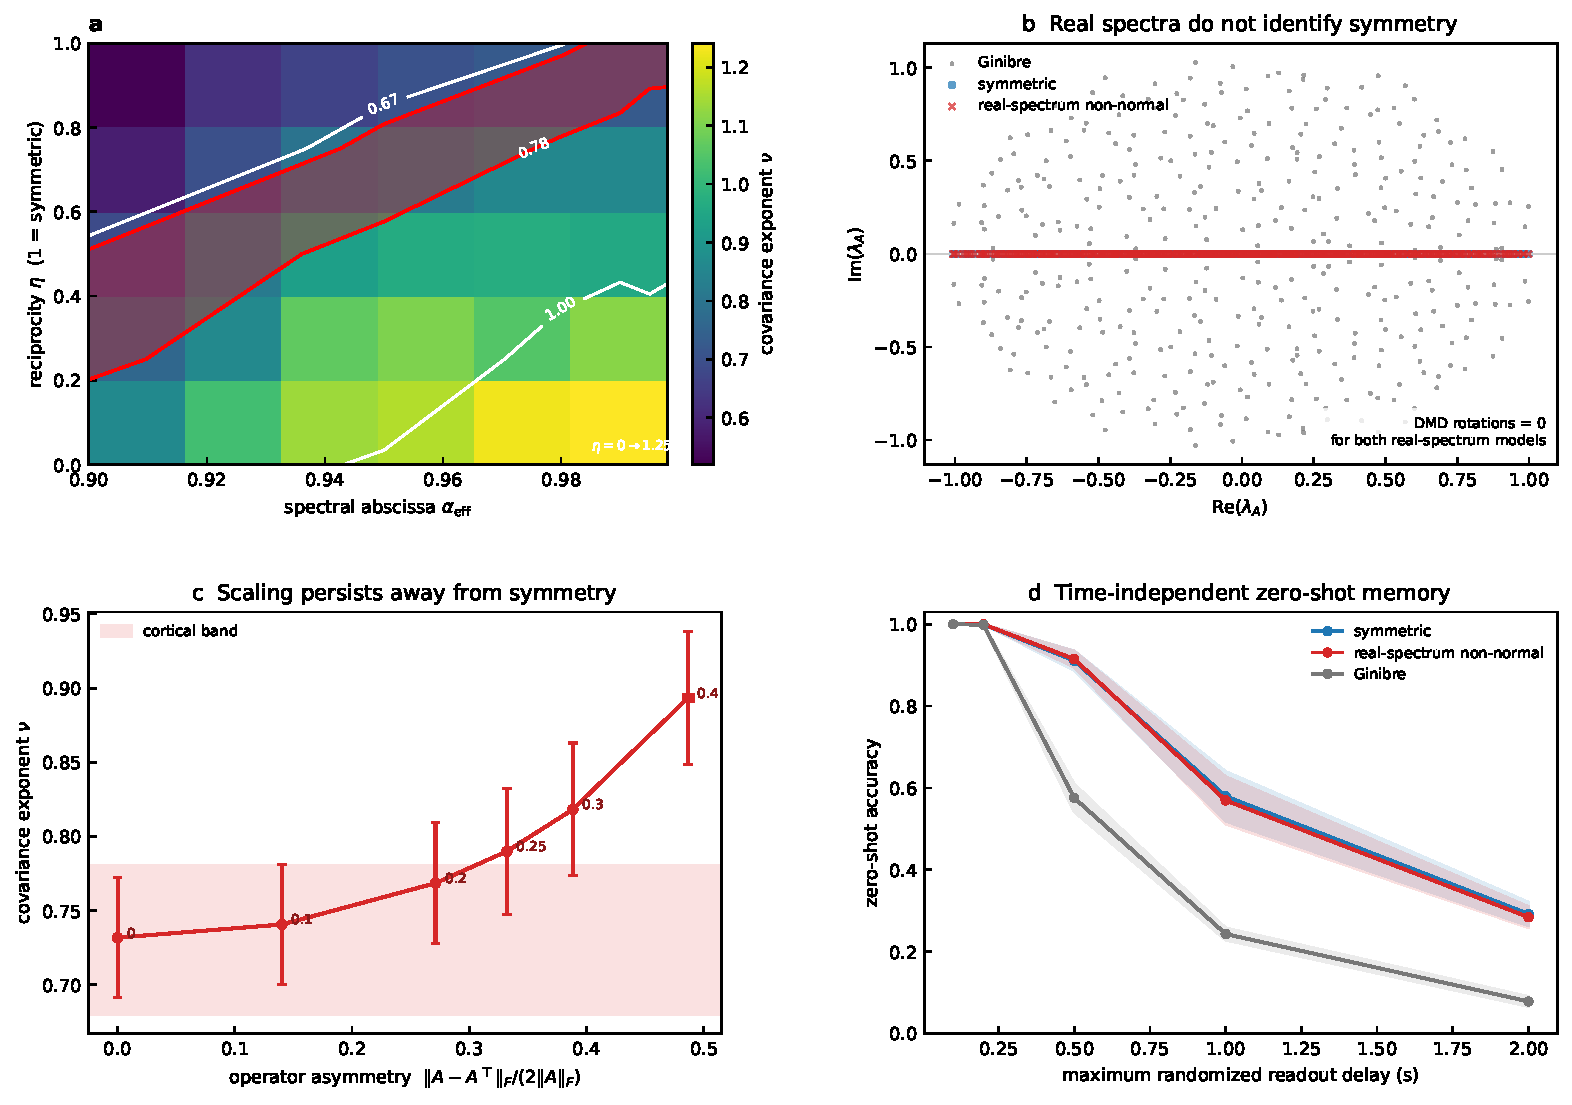
\includegraphics[width=0.98\linewidth]{figures/fig_v4.pdf}
  \caption{\textbf{Two identifiability gaps.}
  \textbf{a}, Continuous-time covariance exponent $\nu(\eta,\alphaeff)$: iso-$\nu$
  contours run diagonally; the cortical band ($0.68$--$0.78$, red) is reproduced
  along a \emph{curve} of (reciprocity $\eta$, spectral abscissa $\alphaeff$)
  pairs, not a point. \textbf{b}, Symmetric and real-spectrum non-normal
  ($A_{0.30}$) operators have identical, entirely real eigenvalues (DMD rotation
  $=0$ for both); a Ginibre control has complex eigenvalues. \textbf{c},
  Covariance exponent $\nu$ versus operator asymmetry as the similarity gain $g$
  grows; the counterexample stays within the Article's reported range up to
  substantial asymmetry. Mean $\pm$ s.d., six realizations. \textbf{d},
  Time-independent zero-shot memory: symmetric and real-spectrum non-normal
  dynamics are indistinguishable ($0.915$ vs $0.911$ at $0.5$\,s); Ginibre
  dynamics degrade sharply.}
  \label{fig:ma}
\end{figure}

\begin{figure}[t]
  \centering
  
\includegraphics[width=0.98\linewidth]{figures/fig_identifiability.pdf}
  \caption{\textbf{Functional readouts do not recover structural reciprocity.}
  Whole-brain \emph{Drosophila} LIF simulations on the
  FlyWire connectome\cite{shiu2024}. Degree-preserving nulls vary structural
  reciprocity $R$ over two orders of magnitude ($0.006$--$0.69$) at fixed
  in/out-degree, weight multiset and Dale sign, bracketing the real value
  ($R=0.265$); the symmetrized null ($R=1$) additionally doubles density.
  \textbf{a}, DMD imaginary content $\max|\Im\lambda|$ is invariant to reciprocity
  ($\approx0.167$, dotted); modal rotation appears only in the synchronous
  high-gain symmetrized regime (stars, rotation $1.4$--$2.0$), where a perfectly
  symmetric graph reads as rotating. \textbf{b}, The covariance exponent $\nu$
  rises with recurrence identically for the real network and both
  degree-preserving nulls; only the density-doubled symmetrized null is flat, so
  its apparent $\nu$ separation reflects density, not reciprocity. Mean $\pm$
  s.d.\ over seeds.}
  \label{fig:flywire}
\end{figure}

\backmatter

\bmhead{Data availability}
Code and numerical outputs reproducing all analyses and figures are available at
\texttt{https://github.com/Mia9469/non-normality}; a versioned archive (Zenodo
DOI) will be cited on acceptance. The FlyWire connectome data are obtained from
the source release of Shiu \emph{et al.}\cite{shiu2024} via the included download
script.

\section*{Declarations}
\noindent\textbf{Competing interests.} The authors declare no competing interests.\\[0.3em]
\noindent\textbf{Author contributions.} All authors designed the analysis,
performed the calculations, interpreted the results, and wrote the
manuscript.\\[0.3em]
\noindent\textbf{Correspondence with the original authors.} A copy of this
comment was provided to the authors of the original Article prior to submission.
\emph{[Replace with their response, or a statement that none was received within
two weeks; attach the correspondence.]}

\bibliography{ma_refs}

\end{document}
